\documentclass{article}
\usepackage{float,amsmath}
\usepackage{graphicx}
\usepackage{color}
\usepackage[letterpaper,margin=1in]{geometry}
\usepackage{hyperref}

%\setlength{\textwidth}{6.5in}

\begin{document}

\author{HERA}
\title{Roadmap for HERA Network Configuration and Bandwidth}
\maketitle

\section{Introduction}
HERA is an international experiment to detect and characterize the Epoch of Reionization (EOR).  The telescope is located at the South African SKA site in the Karoo
Astronomy Reserve.  This brief summarizes the overall network configuration and bandwidth for HERA as relevant to the interfaces with SKA-SA infrastructure.

Figure \ref{fig:hi_level} shows the very high-level network evolution.  Phase 1 (top) currently has a copper/RF connection between the antennas and correlator, which resides in the 'Container' in the middle of the array.  The integrated correlator files are transferred over the local network to processing and storage in the CMC.  The processed files are then transferred to the US, currently to a cluster at the University of Pennsylvania in Philadelphia, PA.  Over the next month or two, the CMC-based equipment will be moved to the KAPB (labelled 'b)') and the US-node will be moved to the National Radio Astronomy Observatory (NRAO) site in Socorro, NM (labelled 'c)').  Current bandwidth and services are adequate for this Phase.

\begin{figure}[H]
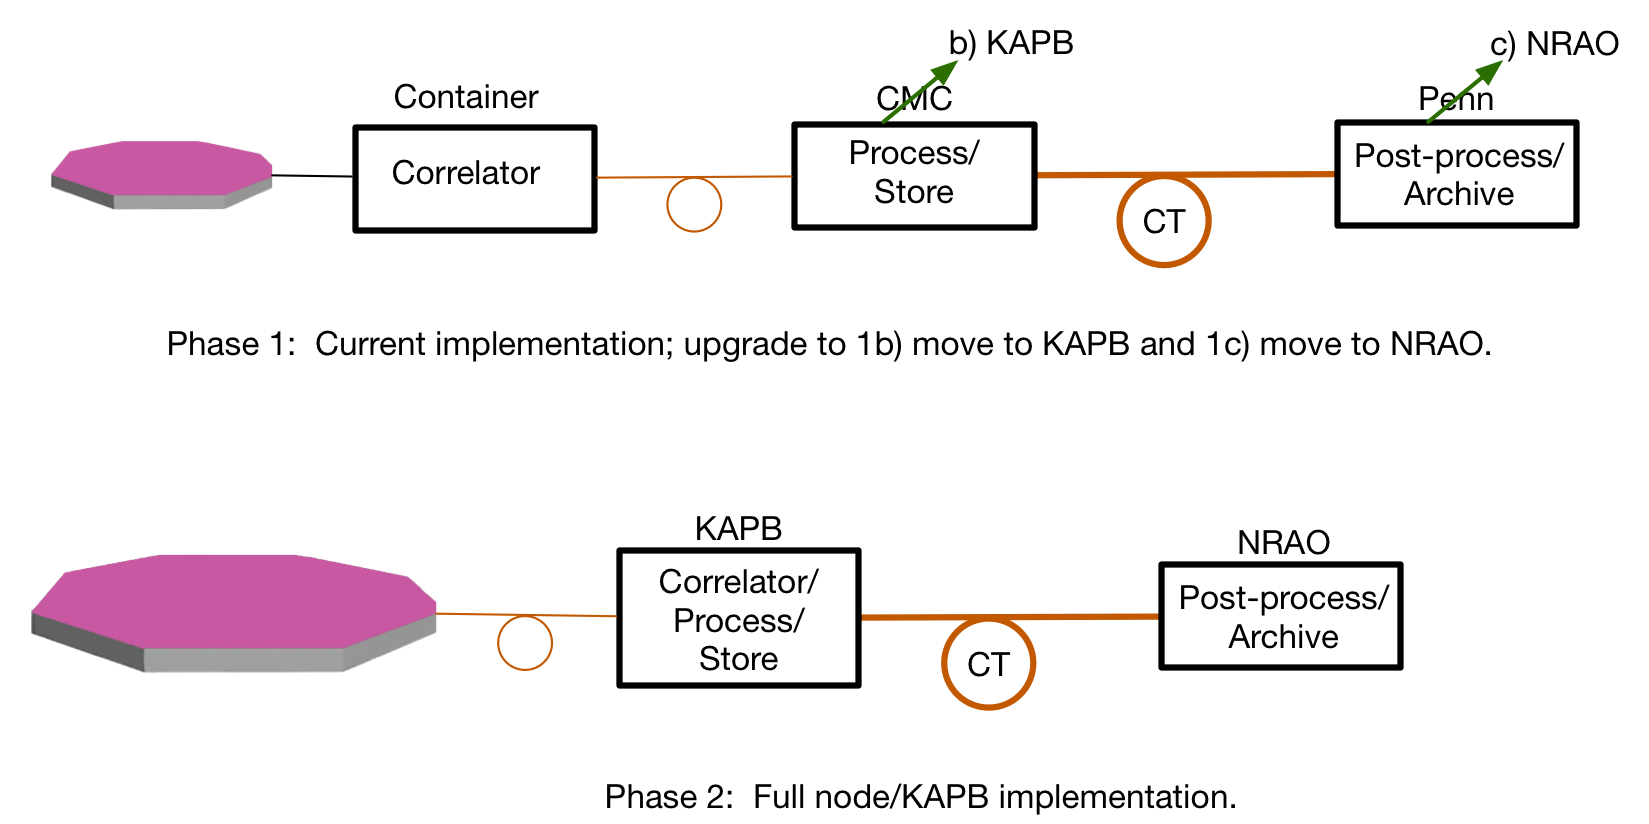
\includegraphics[width=0.8\textwidth]{network.png}
\centering
\caption{High-level organization of network.  See text for explanation.}
\label{fig:hi_level}
\end{figure}

Prior to the move of the equipment from the CMC to the KAPB, there is a desire to change the network configuration to accommodate both new site and new HERA changes in the current network.  There is no strict requirement that this need happen before that move, however it allows the network change to be tested before a major hardware relocation.  When the equipment is relocated to the KAPB additional memory will be added to the system, as well as upgrading the switches.  Fig. \ref{fig:net_org} 




\begin{figure}[H]
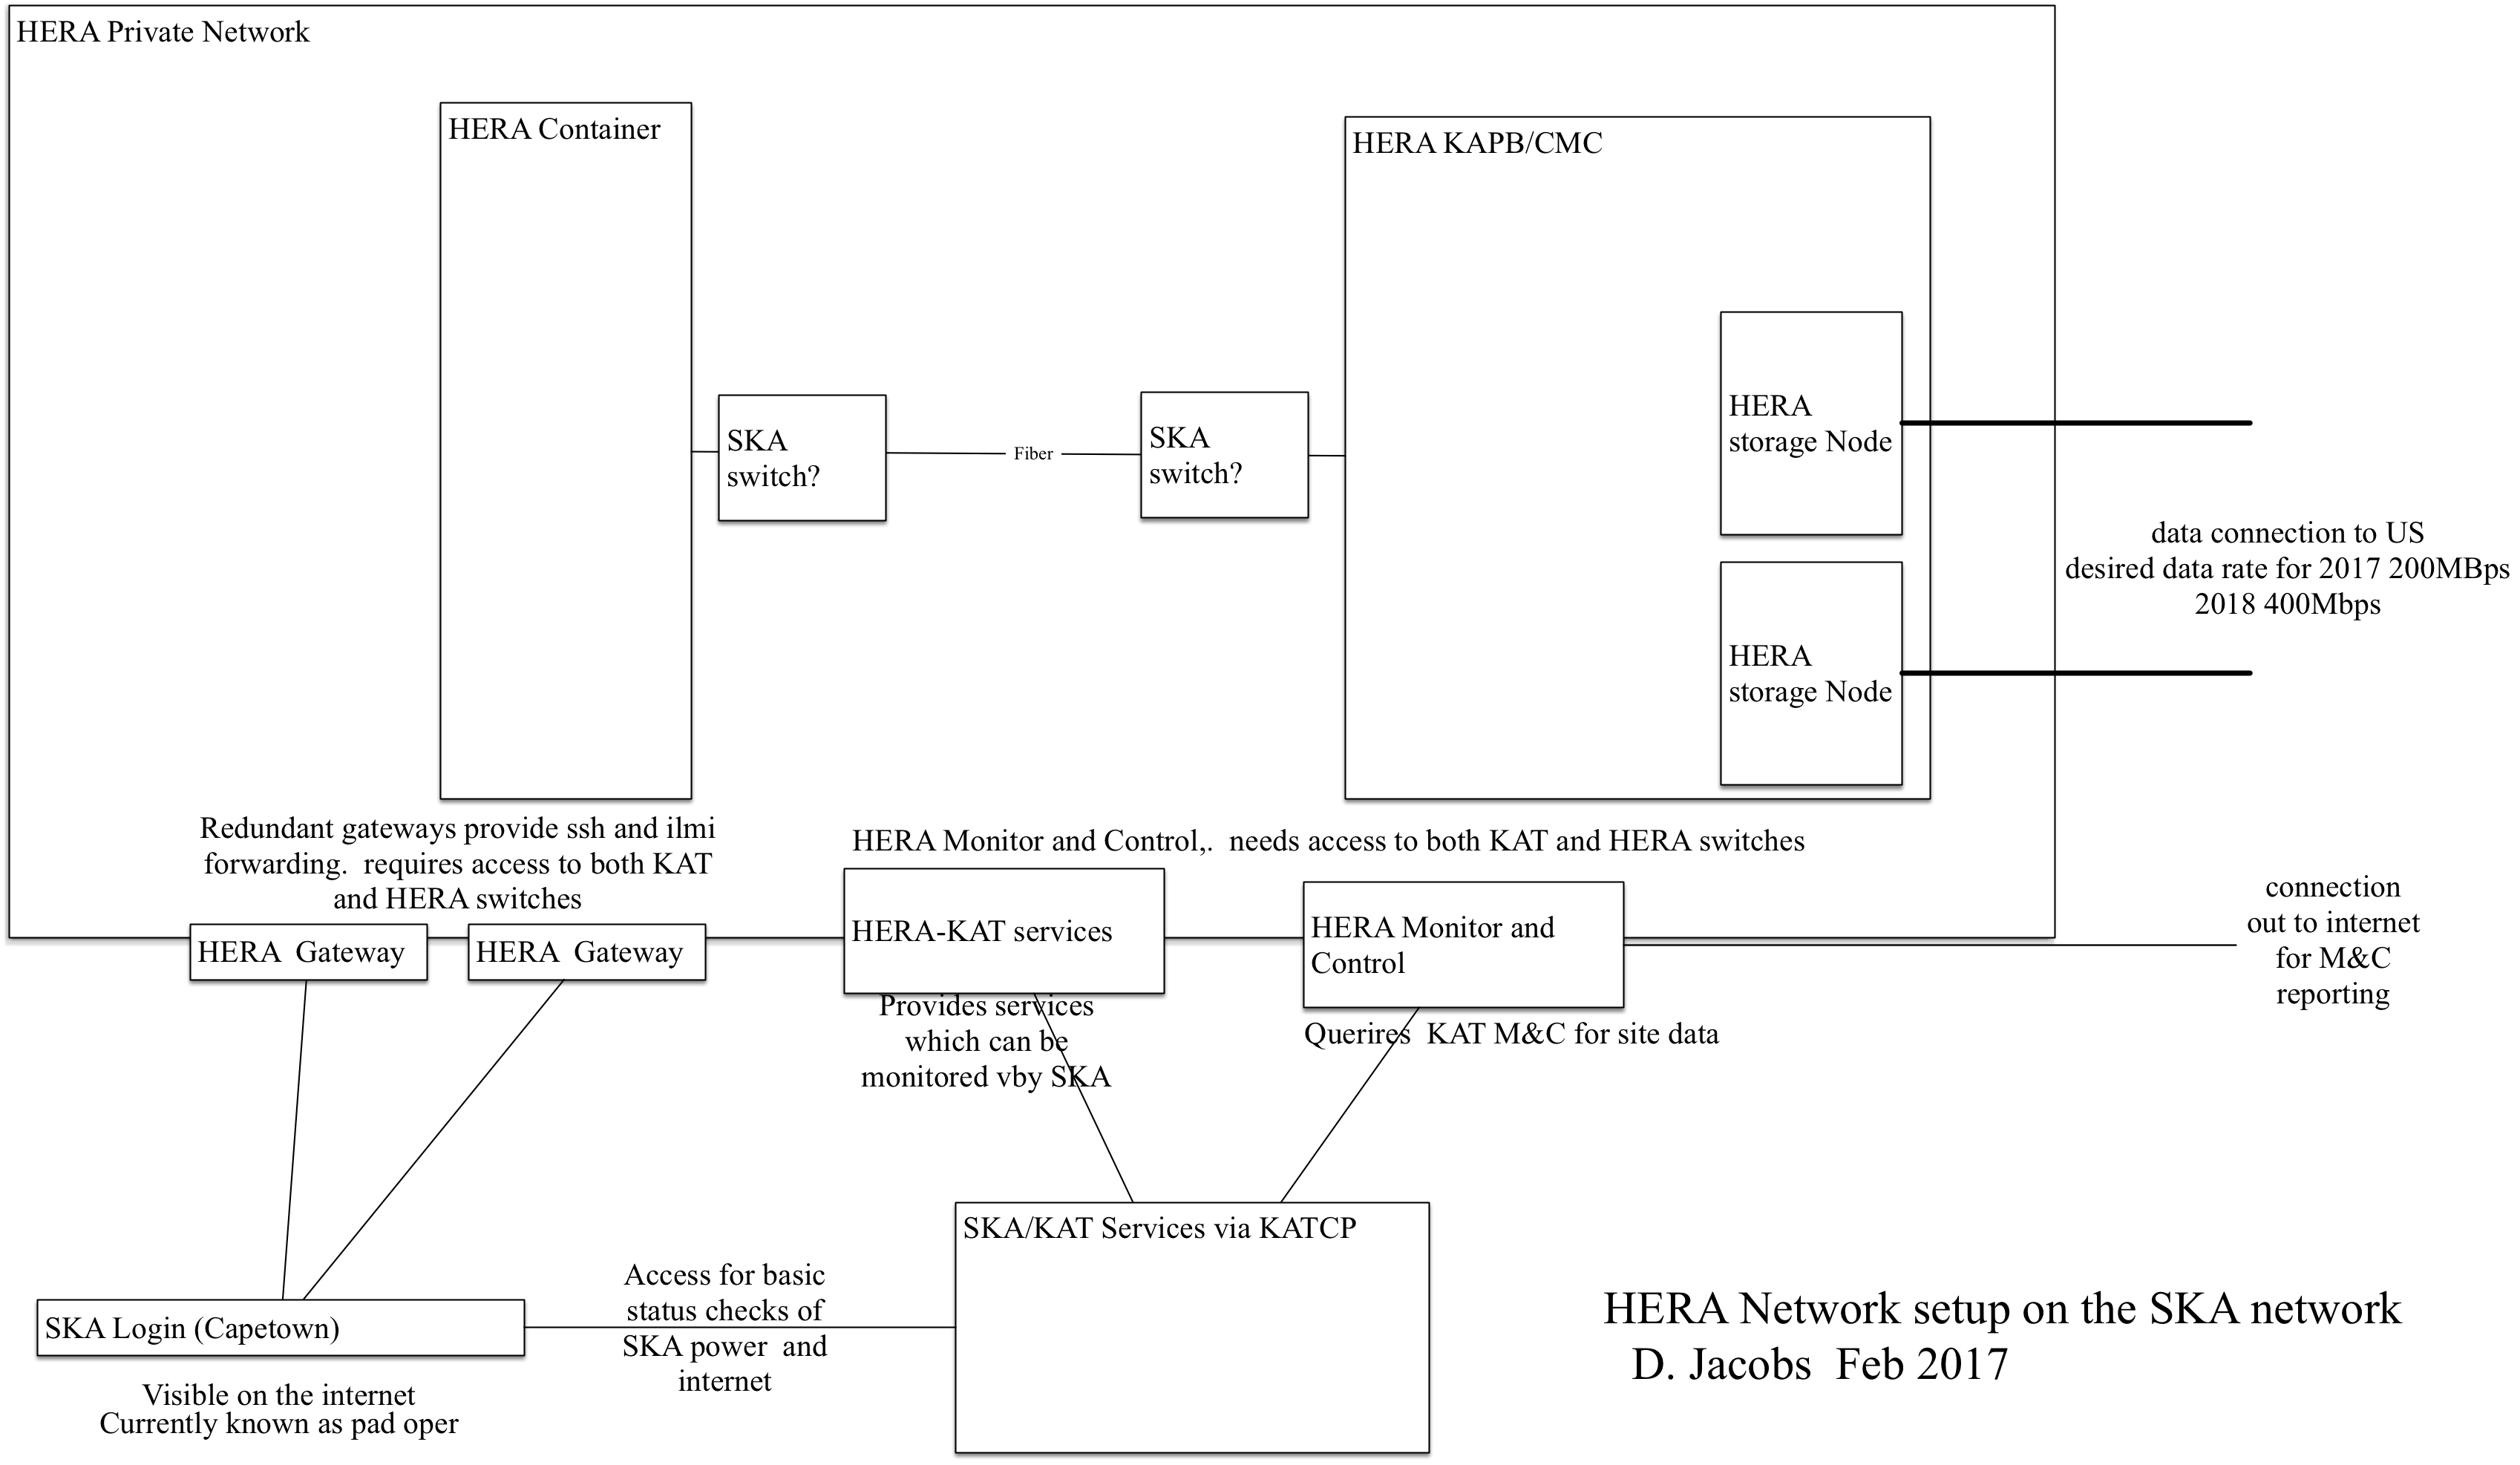
\includegraphics[width=0.8\textwidth]{HERA_2017_network_organization.png}
\centering
\caption{Diagram of modifications to current phase networking.}
\label{fig:net_org}
\end{figure}

\end{document}